\section{Data Visualization}
\begin{itemize}
    \item See trends, clusters and local patterns in data
    \item Difficult to see in raw data
    \item Detect outliers and unusual groups
    \item Validate Hypothesis/Conjecture/Theory
\end{itemize}
\textbf{Important in a Plot}
\begin{itemize}
    \item \textcolor{blue}{X-Axis labels} which data is represented and its units
    \item \textcolor{blue}{Y-Axis labels} which data is represented and its labels
    \item \textcolor{blue}{Title}
    \item \textcolor{blue}{Scale} linear, logarithmic
    \item \textcolor{blue}{Dimensionality of the data 2D / 3D}
\end{itemize}
\textbf{Dataframe}
a two-dimensional labelled data structure with columns of different types

\subsubsection{Data Analysis Libraries}
\textbf{NumPy}
\begin{itemize}
    \item Package for scientific computing in Python
    \item Multidimensional array object
    \item Routines for fast array operations (sorting, selecting, FFT, linear, ...)
\end{itemize}

\textbf{pandas}
\begin{itemize}
    \item Built on top of NumPy
    \item Routines for accessing tabular data from files (.csv, xls, etc.)
    \item Supports 2-dimensional data (dataframe and series)
    \item Dataframes are something like database tables
\end{itemize}

\textbf{MatPlotLib}
\begin{itemize}
    \item Library for visualizing data
    \item Provides bargraphs, histograms, piecharts, scatter plots, lines, boxplots, heatmaps, ...
\end{itemize}

\textbf{Seaborn}
\begin{itemize}
    \item Extension of MatPlotLib, NumPy and pandas
    \item More user friendly
    \item Plots are aesthetically better
\end{itemize}

\subsubsection{Line Plots}
\begin{itemize}
    \item Bivariate, Continuous
    \item Recognizes trend (pattern of change) (over time)
\end{itemize}
\subsubsection{Bar Chart}
\begin{itemize}
    \item Used for categorical data
    \item Counting based on each category
\end{itemize}
\subsubsection{Histogram}
\begin{itemize}
    \item Represents the empirical distribution of a variable
    \item Automatically creates bins (interval) along the range of values
    \item Shows vertical bars to indicate the number of observations per bin
\end{itemize}
\subsubsection{Descriptive Statisics: Box Plots and Violin Plots}
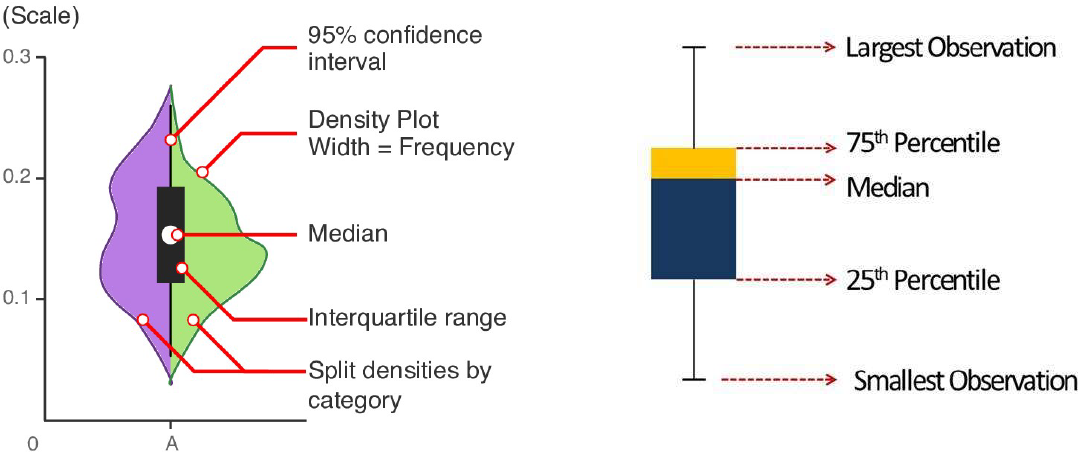
\includegraphics[width=\linewidth]{descriptive_statistics.png}
\subsubsection{Scatter Plot}
\begin{itemize}
    \item Relationship between (two) continuous variables
    \item Helps to get an idea of the degree of correlation between variables
\end{itemize}
